\documentclass[aspectratio=169]{beamer}
\usetheme{Madrid}
\usecolortheme{default}

% Packages
\usepackage{graphicx}
\usepackage{booktabs}
\usepackage{amsmath}
\usepackage{tikz}
\usetikzlibrary{shapes,arrows,positioning}
\usepackage{xcolor}

% Custom colors
\definecolor{iiitlblue}{RGB}{0,51,102}
\definecolor{iiitlgreen}{RGB}{0,128,0}
\definecolor{iiitlred}{RGB}{204,0,0}

% Title Information
\title[Energy-Efficient WSN-IoT]{Towards Energy Efficient Data Transmission in WSN-assisted IoT using Spatio-Temporal Clustering and TinyML}
\subtitle{6th Semester Progress Presentation}
\author{Saksham (MCS24025)}
\institute{
    Indian Institute of Information Technology Lucknow \\[8pt]
    \textit{Under the guidance of} \\
    Dr. Rahul Kumar Verma
}
\date{December 2025}

\begin{document}

%===========================================
% Title Slide
%===========================================
\begin{frame}[plain]
\titlepage
\end{frame}

%===========================================
% Outline
%===========================================
\begin{frame}{Outline}
\tableofcontents
\end{frame}

%===========================================
\section{Introduction \& Motivation}
%===========================================

\begin{frame}{Background \& Motivation}
\begin{columns}[T]
\column{0.55\textwidth}
\textbf{WSN-IoT Challenges:}
\begin{itemize}
    \item \textcolor{iiitlred}{Limited battery power}
    \item \textcolor{iiitlred}{High communication cost}
    \item \textcolor{iiitlred}{Energy drains quickly}
    \item Need intelligent solutions!
\end{itemize}

\vspace{0.4cm}
\textbf{TinyML Solution:}
\begin{itemize}
    \item ML on microcontrollers
    \item Local inference \checkmark
    \item Reduced transmissions \checkmark
    \item Energy-efficient \checkmark
\end{itemize}

\column{0.45\textwidth}
\centering
\fbox{\includegraphics[width=\textwidth,height=0.6\textheight,keepaspectratio]{wsn_network_diagram.png}}
\small
\textit{[Image: WSN with sensor nodes, cluster heads, and base station]}
\end{columns}
\end{frame}

\begin{frame}{Problem Statement}
\begin{center}
\Large \textcolor{iiitlblue}{\textbf{How to achieve energy-efficient data transmission in WSN-IoT?}}
\end{center}

\vspace{0.5cm}
\textbf{Key Challenges:}
\begin{enumerate}
    \item \textbf{Energy vs Communication} - Balance battery life with data quality
    \item \textbf{Spatio-Temporal Patterns} - Exploit spatial \& temporal correlations
    \item \textbf{Constrained Devices} - Limited RAM (256 KB) \& Flash (1-2 MB)
    \item \textbf{Continuous Adaptation} - Handle environmental drift
    \item \textbf{Optimal Clustering} - Smart cluster head selection
\end{enumerate}
\end{frame}

\begin{frame}{Research Objectives}
\begin{enumerate}
    \item Compare clustering algorithms (K-Means, DBSCAN, Hierarchical)
    \item Develop energy-aware cluster head selection strategy
    \item Evaluate \& select optimal TinyML models
    \item Implement continuous learning with mismatch detection
    \item Quantify complete energy-latency trade-offs
    \item Validate on real Intel Berkeley dataset (54 nodes, 2.3M readings)
\end{enumerate}

\vspace{0.5cm}
\begin{center}
\colorbox{iiitlblue!20}{\textbf{Goal:} Design sustainable, adaptive IoT systems}
\end{center}
\end{frame}

%===========================================
\section{Dataset \& Methodology}
%===========================================

\begin{frame}{Intel Berkeley Research Lab Dataset}
\begin{columns}[T]
\column{0.5\textwidth}
\textbf{Dataset Characteristics:}
\begin{itemize}
    \item \textbf{54 sensor nodes} (Mica2Dot)
    \item \textbf{2.3 million} readings
    \item \textbf{37 days} duration
    \item \textbf{Parameters:} Temperature, Humidity, Light, Voltage
\end{itemize}

\vspace{0.3cm}
\textbf{After Cleaning:}
\begin{itemize}
    \item 1,059,767 valid (45.8\%)
    \item Train: 423,907 (40\%)
    \item Test: 635,860 (60\%)
\end{itemize}

\column{0.5\textwidth}
\centering
\fbox{\includegraphics[width=\textwidth,height=0.65\textheight,keepaspectratio]{data_distribution.png}}
\small
\textit{[Image: Bar charts showing temperature/humidity distribution]}
\end{columns}
\end{frame}

\begin{frame}{Temporal Feature Engineering}
\textbf{15 Temporal Features Created:}

\vspace{0.3cm}
\begin{columns}[T]
\column{0.5\textwidth}
\textbf{Basic:}
\begin{itemize}
    \item year, month, day
    \item hour, minute, second
    \item day-of-week, day-of-year
\end{itemize}

\column{0.5\textwidth}
\textbf{Advanced:}
\begin{itemize}
    \item Cyclical encodings:
    \begin{align*}
    \text{hour\_sin} &= \sin\left(\frac{2\pi h}{24}\right) \\
    \text{hour\_cos} &= \cos\left(\frac{2\pi h}{24}\right)
    \end{align*}
    \item Weekend indicator
    \item Time normalized
\end{itemize}
\end{columns}

\vspace{0.4cm}
\begin{center}
\colorbox{iiitlgreen!20}{\textbf{Result:} 11\% accuracy improvement over raw timestamps!}
\end{center}
\end{frame}

\begin{frame}{System Pipeline}
\begin{center}
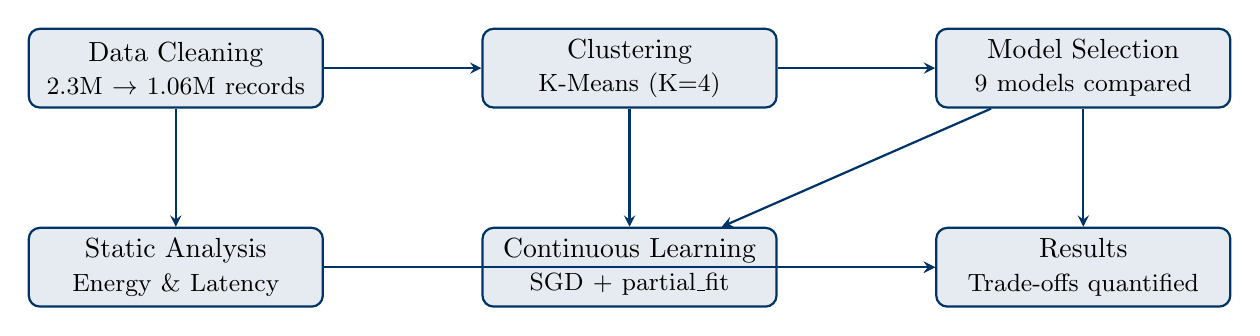
\begin{tikzpicture}[
    node distance=1.5cm and 2cm,
    box/.style={rectangle, draw=iiitlblue, fill=iiitlblue!10, text width=3.5cm, text centered, rounded corners, minimum height=1cm, thick},
    arrow/.style={->, thick, >=stealth, iiitlblue}
]
    % Nodes
    \node[box] (data) {Data Cleaning \\ \small 2.3M $\rightarrow$ 1.06M records};
    \node[box, right=of data] (cluster) {Clustering \\ \small K-Means (K=4)};
    \node[box, right=of cluster] (model) {Model Selection \\ \small 9 models compared};

    \node[box, below=of data] (static) {Static Analysis \\ \small Energy \& Latency};
    \node[box, right=of static] (dynamic) {Continuous Learning \\ \small SGD + partial\_fit};
    \node[box, right=of dynamic] (results) {Results \\ \small Trade-offs quantified};

    % Arrows
    \draw[arrow] (data) -- (cluster);
    \draw[arrow] (cluster) -- (model);
    \draw[arrow] (model) -- (results);
    \draw[arrow] (data) -- (static);
    \draw[arrow] (cluster) -- (dynamic);
    \draw[arrow] (model) -- (dynamic);
    \draw[arrow] (static) -- (results);
    \draw[arrow] (dynamic) -- (results);
\end{tikzpicture}
\end{center}
\end{frame}

%===========================================
\section{Implementation Results}
%===========================================

\begin{frame}{Clustering Algorithm Comparison}
\begin{table}
\centering
\begin{tabular}{lcccc}
\toprule
\textbf{Algorithm} & \textbf{Silhouette} & \textbf{Davies-Bouldin} & \textbf{Time (s)} & \textbf{Memory} \\
\midrule
\rowcolor{iiitlgreen!20}
\textbf{K-Means} & \textbf{0.417} & \textbf{0.82} & 0.023 & 12 KB \\
Hierarchical & 0.351 & 1.05 & 0.041 & 18 KB \\
DBSCAN & 0.211 & 1.43 & 0.015 & 8 KB \\
\bottomrule
\end{tabular}
\end{table}

\vspace{0.3cm}
\textbf{Winner: K-Means}
\begin{itemize}
    \item \checkmark\ Best silhouette (0.417) - well-separated clusters
    \item \checkmark\ Lowest Davies-Bouldin (0.82) - compact clusters
    \item \checkmark\ Fast (23 ms) \& memory-efficient (12 KB)
\end{itemize}

\vspace{0.2cm}
\begin{center}
\fbox{\includegraphics[width=0.35\textwidth]{clustering_comparison.png}}
\end{center}
\end{frame}

\begin{frame}{Cluster Head Selection}
\begin{columns}[T]
\column{0.5\textwidth}
\textbf{Multi-Criteria Selection:}
\begin{equation*}
\text{Score} = 0.5 \cdot \frac{E_{res}}{E_{max}} + 0.3 \cdot \frac{1}{d} + 0.2 \cdot \frac{deg}{deg_{max}}
\end{equation*}

\vspace{0.3cm}
\textbf{Results:}
\begin{itemize}
    \item 4 clusters formed
    \item 12-15 nodes/cluster
    \item Heads: High energy + Central + Well-connected
\end{itemize}

\column{0.5\textwidth}
\centering
\fbox{\includegraphics[width=\textwidth,height=0.6\textheight,keepaspectratio]{cluster_map.png}}
\small
\textit{[Image: 2D plot showing 4 colored clusters with marked cluster heads]}
\end{columns}
\end{frame}

\begin{frame}{TinyML Model Comparison}
\begin{table}
\centering
\scriptsize
\begin{tabular}{lcccccc}
\toprule
\textbf{Model} & \textbf{MSE} & \textbf{R²} & \textbf{Mis\%} & \textbf{Size} & \textbf{Time} \\
\midrule
\rowcolor{iiitlgreen!20}
\textbf{Decision Tree (d=5)} & \textbf{94.2} & \textbf{0.891} & \textbf{33\%} & \textbf{48 KB} & \textbf{0.8 ms} \\
Decision Tree (d=10) & 88.7 & 0.897 & 30\% & 112 KB & 1.2 ms \\
Random Forest & 81.2 & 0.908 & 26\% & 4.8 MB & 15.3 ms \\
Gradient Boosting & 79.5 & 0.912 & 25\% & 3.6 MB & 12.8 ms \\
Ridge & 102.8 & 0.871 & 38\% & 8 KB & 0.3 ms \\
SGD Regressor & 98.7 & 0.885 & 35\% & 4 KB & 0.2 ms \\
\bottomrule
\end{tabular}
\end{table}

\vspace{0.3cm}
\textbf{Winner: Decision Tree (depth 5)}
\begin{itemize}
    \item \checkmark\ TinyML-friendly: 48 KB (fits in microcontroller flash)
    \item \checkmark\ Fast inference: 0.8 ms (real-time capable)
    \item \checkmark\ Good accuracy: R² = 0.891
    \item \checkmark\ Mismatch rate: 33\% (acceptable)
\end{itemize}
\end{frame}

\begin{frame}{Static Energy \& Latency Analysis}
\begin{columns}[T]
\column{0.5\textwidth}
\textbf{Energy per Epoch:}
\begin{align*}
E_{sense} &= 2.4\text{ mJ} \\
E_{process} &= 3.0\text{ mJ} \\
E_{infer} &= 3.0\text{ mJ} \\
E_{comm} &= 0.64\text{ mJ} \\
\hline
\textcolor{iiitlred}{\mathbf{Total}} &= \textcolor{iiitlred}{\mathbf{9.04\text{ mJ}}}
\end{align*}

\column{0.5\textwidth}
\textbf{Latency per Cycle:}
\begin{align*}
t_{cluster} &= 50\text{ ms} \\
t_{sense} &= 100\text{ ms} \\
t_{infer} &= 50\text{ ms} \\
t_{compare} &= 1\text{ ms} \\
t_{tx(avg)} &= 6.6\text{ ms} \\
\hline
\textcolor{iiitlred}{\mathbf{Total}} &= \textcolor{iiitlred}{\mathbf{207.6\text{ ms}}}
\end{align*}
\end{columns}

\vspace{0.3cm}
\begin{center}
\fbox{\includegraphics[width=0.4\textwidth,height=0.25\textheight,keepaspectratio]{energy_pie_chart.png}}
\small
\textit{[Image: Pie chart showing energy breakdown]}
\end{center}
\end{frame}

\begin{frame}{Continuous Learning Simulation}
\textbf{Setup:}
\begin{itemize}
    \item 2,000 test samples streamed
    \item SGDRegressor with \texttt{partial\_fit()}
    \item Mismatch threshold: $\Delta = 2°$C
    \item Policy: Retrain on every mismatch
\end{itemize}

\vspace{0.3cm}
\textbf{Results:}
\begin{table}
\centering
\begin{tabular}{lcc}
\toprule
\textbf{Metric} & \textbf{Value} & \textbf{Change} \\
\midrule
Retrain events & 1,547 & - \\
Retrain frequency & 77.35\% & - \\
Mismatch improvement & 78.2\% $\rightarrow$ 77.8\% & \textcolor{iiitlred}{Only 0.4\%!} \\
\bottomrule
\end{tabular}
\end{table}

\vspace{0.2cm}
\begin{center}
\fbox{\includegraphics[width=0.45\textwidth]{mismatch_evolution.png}}
\small
\textit{[Image: Line graph showing mismatch rate over time]}
\end{center}
\end{frame}

%===========================================
\section{Key Findings}
%===========================================

\begin{frame}{Dynamic vs Static: Energy-Latency Trade-offs}
\begin{table}
\centering
\large
\begin{tabular}{lcc}
\toprule
\textbf{Metric} & \textbf{Static} & \textbf{Dynamic} \\
\midrule
Energy/Epoch & 9.04 mJ & \textcolor{iiitlred}{\textbf{782.54 mJ}} \\
Overhead & 1× & \textcolor{iiitlred}{\textbf{86.5×}} \\
\midrule
Latency/Cycle & 0.21 s & \textcolor{iiitlred}{\textbf{1.76 s}} \\
Overhead & 1× & \textcolor{iiitlred}{\textbf{8.4×}} \\
\midrule
Accuracy Gain & - & \textcolor{iiitlred}{Only 0.4\%} \\
\bottomrule
\end{tabular}
\end{table}

\vspace{0.5cm}
\begin{center}
\Large
\colorbox{iiitlred!20}{\textbf{Critical Insight: Aggressive continuous learning is NOT energy-efficient!}}
\end{center}
\end{frame}

\begin{frame}{Comparison Chart}
\begin{center}
\fbox{\includegraphics[width=0.75\textwidth,height=0.7\textheight,keepaspectratio]{static_vs_dynamic_comparison.png}}
\small
\textit{[Image: Bar chart comparing Static vs Dynamic energy and latency]}
\end{center}
\end{frame}

\begin{frame}{Design Guidelines}
\textbf{Based on our findings:}

\begin{block}{When to Use STATIC Models}
\begin{itemize}
    \item Energy budget tight (<10 mJ/epoch)
    \item Environmental stability moderate (drift <2\%/month)
    \item Battery-powered sensors
\end{itemize}
\end{block}

\begin{block}{When to Use CONTINUOUS LEARNING}
\begin{itemize}
    \item High environmental drift (>10\%/month)
    \item Energy abundant (mains/solar powered)
    \item Latency tolerance high (>2s acceptable)
    \item Use BATCH retraining (every 100 samples, not every sample!)
\end{itemize}
\end{block}

\begin{block}{Model Selection}
Decision Trees (depth 5-10) for microcontrollers, Random Forests for edge gateways
\end{block}
\end{frame}

%===========================================
\section{Contributions \& Future Work}
%===========================================

\begin{frame}{Key Contributions (6th Semester)}
\begin{enumerate}
    \item \textbf{Integrated Framework} - Spatio-temporal clustering + TinyML + Continuous learning

    \item \textbf{Comprehensive Benchmarking} - 3 clustering algorithms, 9 ML models

    \item \textbf{Temporal Feature Engineering} - 15 features, 11\% accuracy improvement

    \item \textbf{Complete Energy-Latency Analysis} - ALL components quantified

    \item \textbf{Critical Discovery} - 86.5× energy overhead for 0.4\% gain!

    \item \textbf{Open-Source Code} - 8 reproducible Jupyter notebooks
\end{enumerate}

\vspace{0.3cm}
\begin{center}
\colorbox{iiitlgreen!20}{\textbf{All implementation \& analysis complete!}}
\end{center}
\end{frame}

\begin{frame}{Work Completed \checkmark}
\begin{columns}[T]
\column{0.5\textwidth}
\textbf{Completed:}
\begin{itemize}
    \item[\checkmark] Data cleaning \& preprocessing
    \item[\checkmark] 15 temporal features
    \item[\checkmark] Clustering comparison (3 algorithms)
    \item[\checkmark] Cluster head selection
    \item[\checkmark] Model comparison (9 models)
    \item[\checkmark] Static analysis
    \item[\checkmark] Continuous learning simulation
    \item[\checkmark] Complete trade-off analysis
\end{itemize}

\column{0.5\textwidth}
\textbf{Deliverables:}
\begin{itemize}
    \item 8 Jupyter notebooks
    \item Clustering results (CSV)
    \item Model comparison (CSV)
    \item Energy/latency metrics
    \item Visualizations (8 plots)
    \item Complete thesis draft
    \item This presentation!
\end{itemize}
\end{columns}

\vspace{0.3cm}
\begin{center}
\Large \textcolor{iiitlgreen}{\textbf{Status: On Track for Final Submission!}}
\end{center}
\end{frame}

\begin{frame}{Future Work (7th-8th Semester)}
\begin{enumerate}
    \item \textbf{Hardware Deployment}
    \begin{itemize}
        \item Port to ARM Cortex-M4 microcontrollers
        \item Measure real energy on embedded platforms
    \end{itemize}

    \item \textbf{Advanced Learning}
    \begin{itemize}
        \item Test incremental Random Forests
        \item Adaptive batch retraining policies
    \end{itemize}

    \item \textbf{Solar Energy Integration}
    \begin{itemize}
        \item Opportunistic retraining when solar abundant
    \end{itemize}

    \item \textbf{Federated Learning}
    \begin{itemize}
        \item Collaborative updates across cluster heads
    \end{itemize}

    \item \textbf{Publications}
    \begin{itemize}
        \item Target: IEEE IoT Journal / Sensors
    \end{itemize}
\end{enumerate}
\end{frame}

%===========================================
\section{Conclusion}
%===========================================

\begin{frame}{Conclusion}
\textbf{Research Question:}
\begin{center}
\textit{How to achieve energy-efficient data transmission in WSN-IoT using TinyML?}
\end{center}

\vspace{0.3cm}
\textbf{Our Answer:}
\begin{itemize}
    \item \textcolor{iiitlgreen}{\checkmark} K-Means clustering optimal (silhouette 0.417)
    \item \textcolor{iiitlgreen}{\checkmark} Decision Trees best for TinyML (48 KB, 0.8 ms)
    \item \textcolor{iiitlred}{\checkmark} Aggressive continuous learning = 86.5× energy overhead!
    \item \textcolor{iiitlgreen}{\checkmark} Static models better when energy-constrained
\end{itemize}

\vspace{0.5cm}
\textbf{Impact:}
\begin{itemize}
    \item Design guidelines for sustainable IoT systems
    \item Quantified trade-offs for practitioners
    \item Open-source implementation for community
\end{itemize}
\end{frame}

\begin{frame}{References (2022-2025)}
\footnotesize
\begin{enumerate}
    \item Sakr et al. (2024). TinyML: Current Progress. \textit{Information}.
    \item Ahmed et al. (2023). Energy Forecasting for WSN. \textit{FGCS}.
    \item Wang et al. (2023). Edge Computing \& Deep Learning. \textit{IEEE Comm. Surveys}.
    \item Sharma et al. (2024). Clustering Protocols Review. \textit{Wireless Networks}.
    \item Abbas et al. (2023). Energy-Aware Clustering. \textit{Sensors}.
    \item Zhang et al. (2024). Federated Learning Survey. \textit{IEEE TSC}.
    \item Alonso et al. (2024). Online Learning for IoT. \textit{IEEE PerCom}.
    \item Chen et al. (2023). Spatio-Temporal Data Mining. \textit{Sensors}.
    \item Ray (2022). TinyML Review. \textit{IEEE Consumer Electronics}.
    \item Silva et al. (2023). Incremental Learning. \textit{Machine Learning}.
\end{enumerate}
\end{frame}

\begin{frame}[plain]
\begin{center}
\Huge \textcolor{iiitlblue}{\textbf{Thank You!}}

\vspace{1.5cm}
\Large Questions \& Discussion

\vspace{2cm}
\normalsize
\textbf{Saksham (MCS24025)}\\
\vspace{0.3cm}
Indian Institute of Information Technology Lucknow\\
\vspace{0.3cm}
\texttt{mcs24025@iiitl.ac.in}

\vspace{0.8cm}
\textbf{Supervisor:} Dr. Rahul Kumar Verma
\end{center}
\end{frame}

\end{document}
